\documentclass[12pt]{article}
\usepackage{polski}
\usepackage[utf8]{inputenc}
\usepackage{amsmath}
\usepackage{anysize}
\usepackage{listings}
\usepackage{graphicx}
\usepackage{color}
\title{Wykorzystanie silników fizycznych na platformach mobilnych}
\author{Mateusz Kortas}
\date{12.05.2012}
\begin{document}
\marginsize{2.5cm}{2cm}{1cm}{1cm}
  \maketitle
  \tableofcontents
  \section{Wstęp}\label{sec:wstep}
  \subsection{Czym jest silnik fizyczny?}\label{subsec:czymJestSilnik}
TODO
  \subsection{Cele projektu.}\label{subsec:celeProjektu}
TODO
  \section{Wykorzystane technologie.}
  \subsection{Android SDK}
TODO
  \subsection{Bullet physics engine}
TODO
Lorem Ipsum jest tekstem stosowanym jako przykładowy wypełniacz w przemyśle
poligraficznym. Został po raz pierwszy użyty w XV w. przez nieznanego drukarza do wypełnienia tekstem próbnej książki. Pięć wieków później zaczął być używany przemyśle elektronicznym, pozostając praktycznie niezmienionym. Spopularyzował się w latach 60. XX w. wraz z publikacją arkuszy Letrasetu, zawierających fragmenty Lorem Ipsum, a ostatnio z zawierającym różne wersje Lorem Ipsum oprogramowaniem przeznaczonym do realizacji druków na komputerach osobistych, jak Aldus PageMaker
  \subsection{Android NDK}
TODO
  \section{Wykorzystanie Bullet physics engine przez Android NDK}
  \subsection{Konfiguracja Android NDK w środowisku Eclipse}
  % [source]http://mhandroid.wordpress.com/2011/01/23/using-eclipse-for-android-cc-development/
  Aby utworzyć projekt Androida z możliwością edycji i kompilacji bibliotek
  natywnych należy: \\
  1. Zainstalować środowisko Eclipse(i doinstalować do niego wtycczkę ADT).\\
  2. Pobrać kolejno Android SDK i NDK. Do edycji plików żródłowych jest
  też konieczne pobranie wtyczki CDT(C++ Development Tools). Potrzebny będzie
  rónież kod żródłowy biblioteki bullet. Dodatki w eclipse instaluje się przez
  Help -> Install new software\ldots , wpisując adres http://download.eclipse.org/releases/galileo (lub zamisat
  galileo wpisać nazwę swojej wersji Eclipse).
  
  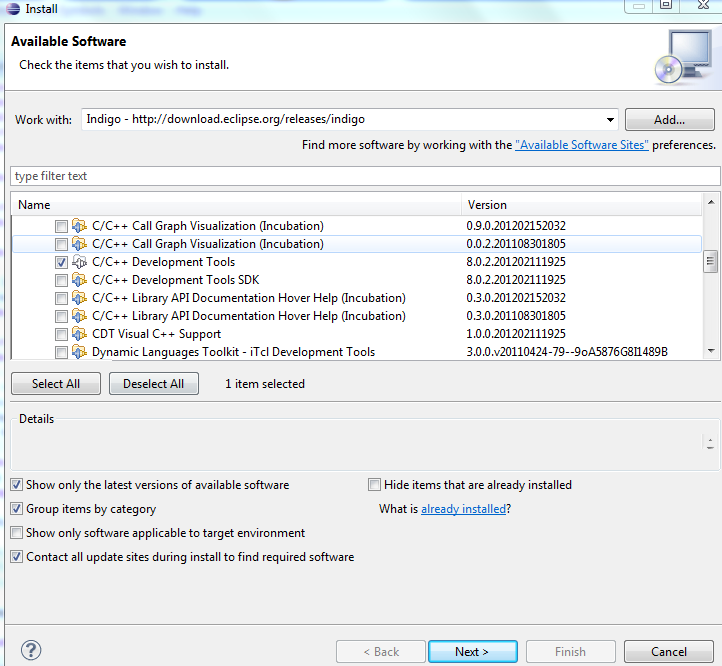
\includegraphics[width=\textwidth]{./img/CDT.png}
  3. Utworzyć nowy standardowy projekt aplikacji na system Android.\\
  4. Do projektu dodać folder jni gdzie przechowywany będzie kod źródłowy w
  języku C++. Skopiować do niego foldery z kodu źródłowego biblioteki
  bullet(będą potrzebne biblioteki BulletCollision, BulletDynamics i
  LinearMath, a także pliki btBulletCollisionCommon.h,
  btBulletDynamicsCommon.h, Bullet-C-Api.h).
  
  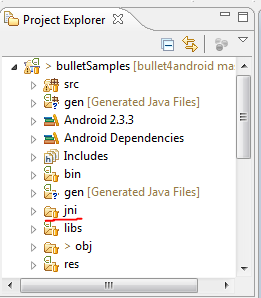
\includegraphics{./img/jni-folder.png}
  
  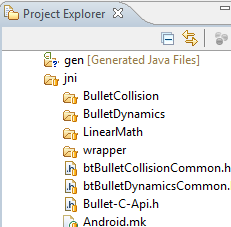
\includegraphics{./img/bulletFoldery.png}
  
  5. Umieścić w folderze plik Android.mk . Zawiera on informacje jak powinien
  być zbudowany projekt w kodzie natywnym. Do tego pliku należy
  dodać informacje o plikach źródłowych biblioteki bullet.
  \lstinputlisting[language=make, caption=Zawartość pliku Android.mk,
  label=andMake,
  breaklines=true,numbers=left,frame=single]{./listings/bulletMkfile.mk}
  
  6. Przekonwertować projekt java na java/C++ , przez menu File -> New ->
  Other\ldots
  
  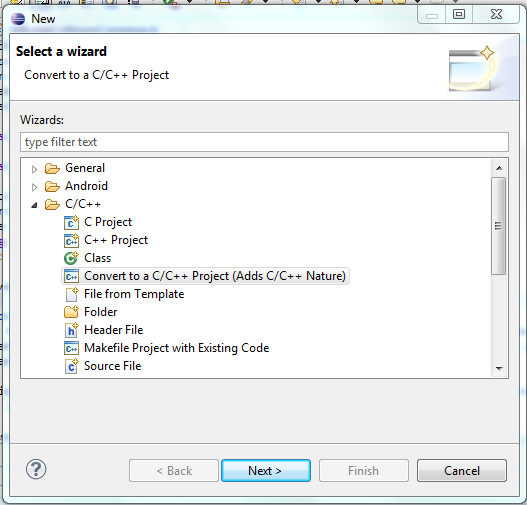
\includegraphics{./img/convert.png}
  
  7. W Properties projektu ustawić budowanie kodu w C++ przez ndk-build.
  Najlepiej miejsce rozpakowania Android NDK przypisać pod zmienną środowiskową
  (np. NDKROOT), co ułatwi przenośność projektu.
  
  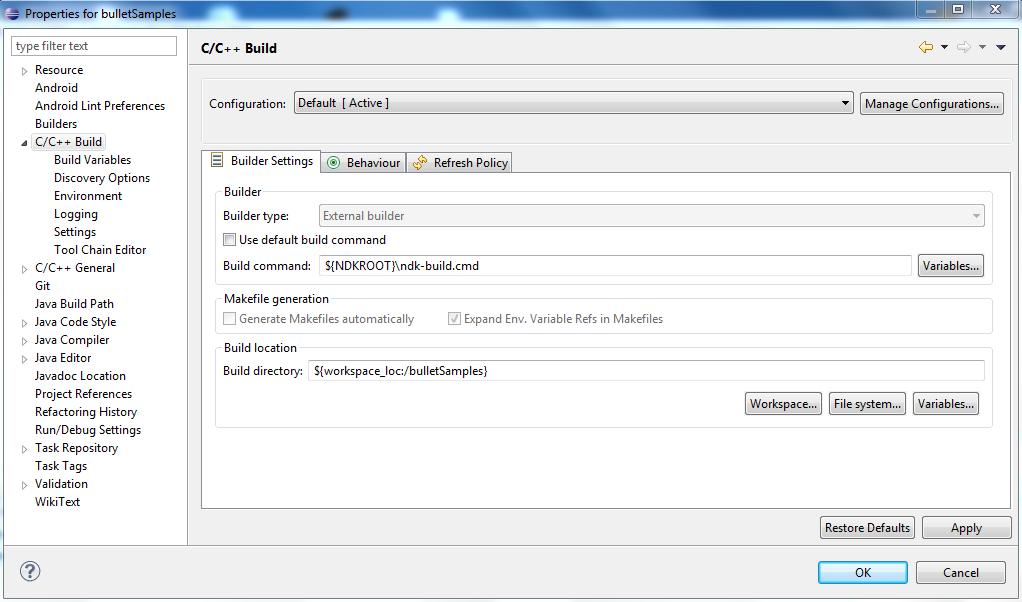
\includegraphics[width=\textwidth]{./img/properties.png}
  
  W zakładce behavior należy odznaczyć checkboxa Clean i usunąć tekst z pola
  Build.\\
  8. W C++ General -> Paths And Symbols dodać ścieżkę dla nagłówków.
  {NDKROOT}\backslash platforms\backslash
  android-14\backslash arch-arm\backslash usr\backslash include
  
  9. Ponieważ w projekcie będą wykorzystywane elementy biblioteki STL, konieczne
  jest dodanie odpowiedniej ścieżki.\\
  
  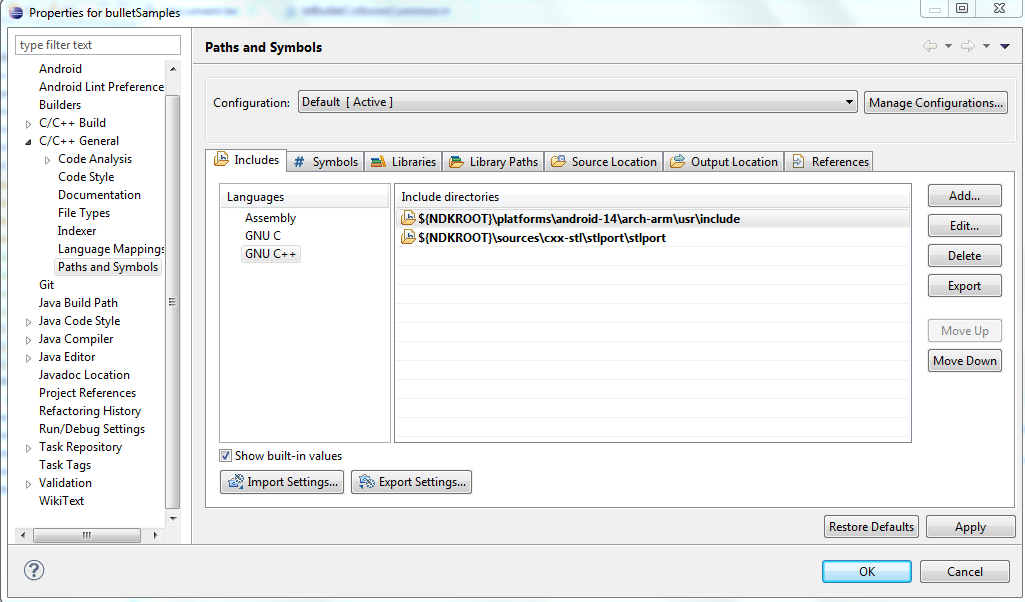
\includegraphics[width=\textwidth]{./img/ndkroot.png}
  
  Dodać również należy informację o wykorzystaniu STL w pliku
  Application.mk(który również muisi być dodany do projektu).
  
  \lstinputlisting[language=make, caption=Zawartość pliku Application.mk,
  label=andMake,
  breaklines=true,numbers=left,frame=single]{./listings/Application.mk}
  
  Po tych czynnościach można edytować projekt ze składnią Javy jak i C++,
  korzystając z autouzupełniania i jednolitej kompilacji. Należy jednak
  pamiętać, że przy dodawaniu nowego pliku z kodem źródłowym w C++ do folderu
  jni konieczne jest umieszczenie o nim informacji w Android.mk .
  \subsection{Zbudowanie biblioteki Bullet na platformę ARM.}
Budowę biblioteki Bullet na platformę Android rozpoczyna się od stworzenia odpowiednika pliku makefile - Android.mk. Należy skopiować źródła bibliotek LinearMath, BulletCollision oraz BulletDynamics do folderu jni w głównym folderze projketu. Następnie dodać do pliku Android.mk informacje o plikach z kodem tych bibliotek, jak to przedstawia listing \ref{andMake}.

Na końcu pliku umieszczamy również listę plików własnej biblioteki(wrappera). Niezbędnym jest również umieszczenie w pliku Application.mk informacji o tym, że przy kompilacji używany będzie pakiet STL.

Do kompilacji używamy aplikacji ndk-build.cmd znajdującej się w pakiecie Android NDK.

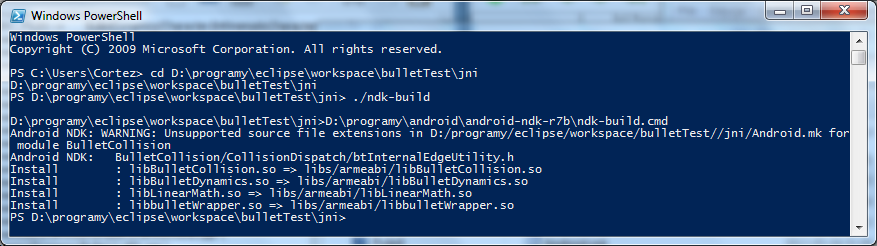
\includegraphics[width=\textwidth]{./img/ndk-build.png}

\subsection{Wywoływanie funkcji natywnych z poziomu Javy.}

\subsection{Konserwacja obiektów.}

\subsection{Przekazywanie argumentów i zwracanych wartości.}

\end{document}
%http://java.sun.com/docs/books/jni/html/refs.html
